\documentclass[]{aiaa-tc} % insert '[draft]' option to show overfull boxes

 \title{An application of Graph Theory to MDAO problem formulation}
        
\author{
  David Pate, %
     \thanks{Georgia Tech}
  Dr. Brian German 
     \thanks{Georgia Tech...}
  Justin Gray,%
     \thanks{Aerospace Engineer, MDAO Branch, Mail Stop 5-11, AIAA Member}   
 }
 
%\usepackage{setspace}
%\doublespace

\usepackage{graphicx}
\usepackage{wrapfig}
\usepackage{caption} 
\usepackage{amsmath}
\usepackage{lscape}
\usepackage{hyperref}
\usepackage{appendix}
\usepackage[section]{placeins}

\captionsetup[figure]{margin=5pt,font=small,labelfont=bf,textfont=bf,justification=justified,}
%\captionsetup[wrapfigure]{margin=5pt,font=small,labelfont=bf,justification=justified,singlelinecheck=off}
\captionsetup[table]{margin=5pt,font=small,labelfont=bf,textfont=bf,justification=justified,position=top}

\bibliographystyle{aiaa}

\usepackage{lettrine}
\usepackage{verbatim}

%\usepackage{hyperref} %allows for the creation of actual text links
\begin{document}

\maketitle
 
\begin{abstract}
   blah blah blah
\end{abstract}

\section*{Nomenclature}

\begin{tabular}{l l} 
    AAO      & All-At- \\
    MDAO     & Multidisciplinary Design Analysis and Optimization \\
    FPF      & Fundamental Problem Formulation \\
\end{tabular}


\section{Introduction}
    
    As the size and complexity of engineering systems grows the time and expense for setting up 
    analysis models grows with them. Multidisciplinary Design Analysis and Optimization (MDAO)
    frameworks such as OpenMDAO\cite{Gray2012} and ModelCenter have enabled a new level of analysis tool integration 
    and paved the way for models of with more analysis tools and increasing numbers of multidisciplinary couplings. 
    Such complex models present a distinct challenge proper implementation of any given solution strategy . 
    In fact as the size of a problem grows very large even selecting an appropriate solution strategy can be a daunting 
    task. 

    To help address in order to address the complexity problem we propose the use of graph based problem formulation 
    in a way that allows for both analysis of potential solution strategies and automated implementation of those strategies 
    inside an MDAO framework. In order to serve that purpose, the problem  needs to include the following information: 
    \begin{itemize}
       \item Discipline Analyses 
       \item Discipline State Variables and Residuals
       \item Design Variables
       \item Constraints
       \item Objective or Objectives
       \item Coupling Constraints
       \item Parameters
    \end{itemize}
    Notably absent from the preceding list are any kind of solvers, optimizers, or other iterative solution finding tools. 
    At it most basic, a problem formulation includes only information about what is being sought after in a given problem, or what the
    goals of a given problem are. It need not contain any information about solution paths or strategies to reach those goals. 
    A general specification is one that states nothing specific about a problem solution path. 

    We define a complete and general problem specification striped down to it's most essential parts to be the 
    Fundamental Problem Formulation (FPF). By definition, the FPF for any given problem will be constant regardless 
    of which MDAO framework, optimization architecture, optimizer, or solver is used to solve the problem.

    In this work we proposed a graph based syntax for the specification of problem formulation. This graph based syntax provides several key
    features that make it useful for working with large scale MDAO problems. It provides a rigid structure that can be easily manipulated 
    with a wide range of well establish graph-theory algorithms for the purposes of problem decomposition. The graph syntax also 
    provides a means for algorithmically testing a given problem formulation to check if it is the FPF, and if not, to reduce it to the FPF. 
    Lastly, a graph based specification for problem formulation lends itself well to interacting with MDAO frameworks which dramatically 
    increases it's utility for real world applications. 


\section{Fundamental Problem Formulation}
    Problem formulation is most commonly given in a mathematical syntax. For a simple, notional problem the problem formulation
    can be given as follows:  

    \begin{align}
        given & \ \ A.f\left(A.x,A.y\right) \notag
        \\ & \ \  B.f\left(B.x,B.z\right) \notag
        \\ & \ \  C.f1\left(A.f,B.f,C.s\right) \notag
        \\ & \ \  C.f2\left(A.f,B.f,C.s\right) \notag
        \\min &\ \ F\left(C.f1\right) \notag
        \\ w.r.t. &\ \  A.x,A.y,B.x,B.z \notag
        \\ s.t. &\ \ G1\left(A.x,B.z\right) \leq 0 \notag
        \\      &\ \ G2\left(A.y\right) \leq 0 \notag
        \\      &\ \ E\left(A.y,C.f1\right) = 0 \notag
        \\      &\ \ R\left(C.s,C.f2\right) = 0 
        \label{eqn:simple}
    \end{align}

    Where $A,B,C$ represent analysis tools, $F,G1,G2,E,R$ are objective and constraint functions, and each analysis tool 
    has a set of input and output variables. While this does represent a complete problem formulation, 
    it's not the fundamental one since some assumptions have inherently been made about the solution 
    strategy. $C$ is directly dependent
    $A.f$ and $B.f$ as it's inputs. This implies that first you must run $A$ and $B$, then $C$ and
    iterate on the design variables in $A$ and $B$ until you satisfy $E$. However, a different solution could be equally valid and still represent
    the same fundamental problem: 

    \begin{align}
        given & \ \ A.f\left(A.x,C.f1\right) \notag
        \\ & \ \  B.f\left(B.x,B.z\right) \notag
        \\ & \ \  C.f1\left(C.y,B.f,C.s\right) \notag
        \\ & \ \  C.f2\left(C.q,B.f,C.s\right) \notag
        \\min &\ \ F\left(C.f1\right) \notag
        \\ w.r.t. &\ \  A.x,A.y,B.x,B.z \notag
        \\ s.t. &\ \ G1\left(A.x,B.z\right) \leq 0 \notag
        \\      &\ \ G2\left(A.y\right) \leq 0 \notag
        \\      &\ \ E\left(A.f,C.q\right) = 0 \notag
        \\      &\ \ R\left(C.s,C.f2\right) = 0 
        \label{eqn:simple_2}
    \end{align}

    Equation \ref{eqn:simple_2} differs only slightly from Eqn. \ref{eqn:simple}. $A$ is now directly dependent on the output of $C$, 
    and the constraint $E$ has changed as well. Now the problem must be solved by running $B$ and $C$, then $A$ and iterating 
    on the design variables in $B$ and $C$ until you satisfy $E$. Since the formulations in Eqn. \ref{eqn:simple} 
    and \ref{eqn:simple_2} both describe the same problem there must be a more fundamental description of the problem that is common
    between them. We present the FPF as follows: 

    \begin{align}
        given & \ \ A.f\left(A.x,A.y\right) \notag
        \\ & \ \  B.f\left(B.x,B.z\right) \notag
        \\ & \ \  C.f1\left(C.y,C.r,C.s\right) \notag
        \\ & \ \  C.f2\left(C.q,C.r,C.s\right) \notag
        \\min &\ \ F\left(C.f1\right) \notag
        \\ w.r.t. &\ \  A.x,A.y,B.x,B.z \notag
        \\ s.t. &\ \ G1\left(A.x,B.z\right) \leq 0 \notag
        \\      &\ \ G2\left(A.y\right) \leq 0 \notag
        \\      &\ \ E\left(A.f,C.\right) = 0 \notag
        \\      &\ \ R\left(C.s,C.f2\right) = 0 
        \label{eqn:simple_2}
    \end{align}

    \section{Problem Formulation Syntax}

    The same mathematical syntax can be used to describe more complex problem formulations
    such as ones that would decompose the FPF to a set of sub-problems. Tedford and Martins used this format to specify the 
    FPF for a set of test problems and also to describe specific formulations for solving them with a 
    number of optimization architectures\cite{Tedford2009}. Their work demonstrates clearly how multiple specific 
    problem formulations can all relate back to a common FPF. 

    In the above problem formulation, there is no explicit relationship definition of local and global features. Instead they are 
    implicitly defined through variable naming conventions. For instance, $x$ is a global variable because it is used in $A.x$ and $B.x$. 
    Simliarly, $A.y$ is a local variable because it only affects the of $A$. If such a naming convention is not in place, 
    then a more explicit definition of the relation between variables must also be given in the form of additional equality constraints between 
    input variables. Similarly, both the constraint, $C$ and the residual, $R$ are presented as equality constraints. They could be classified as 
    a global and a local constraint on the problem respectively, with the only difference being the number of analysis tools that affect them.  
    Hence, the distinction between local and global properties are not necessary to form a fundamental 
    problem formulation. On the other hand, they are relevant when deriving a specific solution path for a problem, so any definition of problem 
    formulation should include the capability to detect the weather a given property is local or global. 

    The challenge with using this traditional mathematical syntax is that it is not easily manipulated or analyzed. 
    A number of matrix based methods have been used successfully to translate the mathematical syntax into a more useful computational form. 
    Steward's Design Structure Matrix (DSM) is a square adjacency matrix which captures the relationship between analysis tools where off 
    diagonal elements of the matrix indicate coupling\cite{Steward1981}. Figure \ref{fig:dsm_simple} shows a DSM for the above notional example. 
    The DSM has been successfully applied in a number of ways to algorithmically modify problem formulations to 
    improve computational efficiency. Rogers et. al developed DeMAID to manipulate a
    DSM  minimizing the computational costs of solving highly coupled systems\cite{Rogers1996}. Notice however, that the DSM in 
    Figure \ref{fig:dsm_simple} contains less information than the full problem formulation. Objective and constraint information 
    is missing and it's not possible to distinguish individual variables.

    \begin{figure}[!hbp]
        \begin{center}
        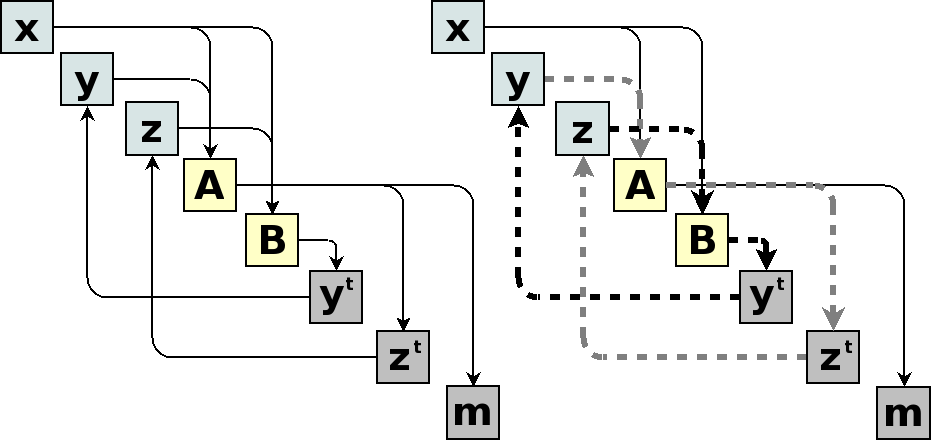
\includegraphics[width=.75\textwidth]{images/dsm_simple}
        \caption{Graph and matrix based DSM specifications for a notional analysis \label{fig:dsm_simple}}
        \end{center}
    \end{figure}

    Since a DSM describes a square adjacency matrix, it can be represented in an equivalent directed graph where nodes represent analysis tools and 
    edges represent information exchange between those tools. An alternate matrix based syntax, called a 
    Functional Dependence Table (FDT), was proposed by Michelena and Papalambros. 
    FDT represents the relationship between functions, including objectives and constraints, and their values\cite{Michelena1997}. Similar to DSM
    FDT also describes an adjacency matrix of a graph. Unlike the DSM graph, however, a FDT graph is an undirected 
    graph where nodes can represent analysis tools, objectives, or constraints. Edges between nodes represent a dependence on the same 
    variable value. By searching the FDT graph for clusters of totally connected nodes Wagner and Papalambros were identify groups of 
    analysis tools that were all dependent on the same input variables and used that to make partitioning decisions \cite{Wagner1993}. FDT retains 
    a greater portion of the information in the problem formulation, but it is still not complete. It ignores information about feedback coupling 
    between codes. 

    It is possible to combine the syntax of an FDT and a DSM by making a small extension to a traditional DSM specification. Normally, a DSM is given 
    with analysis tools as nodes and variable dependencies given as edges. Lamb and Martins included the variables, objectives, and constraint functions
    as nodes in an Extended DSM (XDSM)\cite{Lambe2012} in order to capture a more complete problem formulation for MDAO problems. With XDSM 
    it is possible to specify a complete problem formulation. Lu and Martins developed a process to perform ordering and partitioning on the fundamental 
    problem formulation specified by XDSM in order to achieve significant reductions in computational costs for large scale optimization problems. 
    Figure \ref{fig:dsm_full} illustrates the same notional analysis as in Figure \ref{fig:dsm_simple} represented as an XDSM.

    \begin{figure}[!hbp]
        \begin{center}
        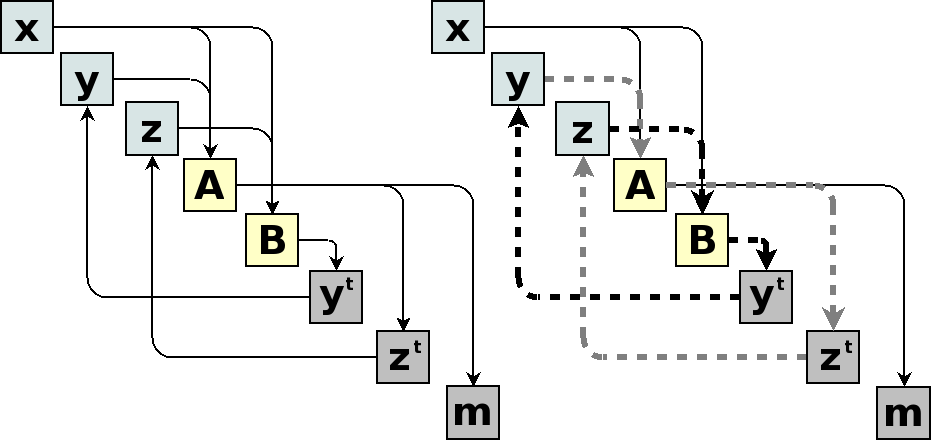
\includegraphics[width=.75\textwidth]{images/dsm_simple}
        \caption{[TODO: Generate XDSM]Extended DSM graph for a notional analysis \label{fig:dsm_full}}
        \end{center}
    \end{figure}

    
\section{Graph--based Problem Formulation Syntax}
A problem formulation will be represented by nodes and edges which will be assigned certain properties and rules. There are many MDAO problem formulation concepts that we wish to represent. An analysis code should be represented by a distinct structure to distinguish between the input, output, and function evaluation, processes. The variables passed between analysis codes should be represented separately to provide insight and control over the dataflow. For example, it is important to distinguish between the case where two analysis codes are supplying the same variable to a third code, or the case where the two analysis codes are providing different variables to the third code. 
Local inputs, local outputs, and design variables(??) should be distinguished from global inputs, which are input that are used by multiple analysis codes.
Objectives and constaints should be represented as separate from local variables because they must be provided in order for the problem formulation to be valid. The coupling between sets of analysis codes is important to capture, and multi--fidelity analysis should also be allowed.

\subsection{Graph Theory Basics}
We begin by discussing the general syntax of graph theory and then expand upon this syntax to represent the data flow of an MDAO problem. The present notation is adapted from Diestel \cite{Diestel2010}.
A \emph{graph} is a pair $G = (V,E)$ of sets such that $E \subseteq V \times V$, which means that the elements of $E$ are 2--element subsets of $V$. The set $V$ contains the \emph{vertices} or \emph{nodes} and the set $E$ contains the \emph{edges}.
For a \emph{directed graph*} we construct $E$ as a set of ordered pairs instead of a set of sets. Each ordered pair represents an edge starting at the node indicated by the first entry and directed to the node indicated by the second entry. Edge $e$ = $(x,y)$ may be referred to simply as $xy$ and we say $y = E(x)$. 
\begin{figure}[htb!]
	\begin{center}
	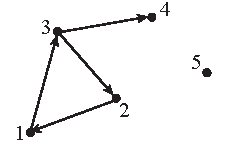
\includegraphics[width=1.5in]{images/example_directed_graph}
	\end{center}
	\vspace{-20pt}
\caption{Example directed graph.}
\label{f:example directed graph}
\end{figure}
As an example, for the directed graph shown in Fig.~\ref{f:example directed graph} we have
\begin{IEEEeqnarray*}{rCl}
V & = & \{1,2,3,4,5\}, \\
E & = & \big\{(1,2),(3,2),(1,3),(3,4)\big\}.
\end{IEEEeqnarray*}

% \subsection{Problem Formulation Concepts to Represent}
% The MDAO problem formulation concepts we wish to represent are:
% \begin{description}
% \item[global input] A global input is a variable that is taken as given and is used by multiple analyses.
% \item[design variable]
% \item[function call] A function call requires a set of inputs to be fulfilled and has certain properties, such as run time, which are independent of the number of outputs actually being used.
% \item[passing of distinct variables] Instead of connecting analyses, the individual variables as are connected
% \item[objective \& constraint] These are variables that must be produced by the problem formulation for it to be valid
% \item[collision] A collision occurs when an input has multiple sources
% \item[hole] A hole occurs when an input has no sources
% \item[coupling] Couple is the mutual dependence between a set of analysis
% \item[multi--fidelity] It may be desirable for the same variable to be calculated by separate analyses and to use both results.
% \end{description}

\subsection{Graph Theory Representation of a Problem Formulation}
In order to represent the listed problem formulation concepts with a graph, we assign properties and rules to nodes and edges.
The first property assigned to nodes and edges is the \emph{type}. \\
The possible node types are:
\begin{description}
\item[variable node] The variable node represents passing of data.
\item[model node] The model node represents the handling of data.
\end{description}
The possible edge types are:
\begin{description}
\item[fixed edge] A fixed edge may not be removed.
\item[free edge] A free edge may be removed.
\end{description}
Model nodes must be used with the following rules:
\begin{itemize}
\item A model node can only have one edge directed to or from another model node.
\item A model node can only have fixed edges directed in or out.
\item A model node must have at least one edge directed in and at least one edge directed out.
\end{itemize}
The MDO problem formulation concepts represented by nodes are given in Table \ref{t:node representation}, and the concepts represented by nodes are given in Table \ref{t:edge representation}.
% \begin{itemize}
% \item An objective or constraint is indicated by a variable node with no outgoing edges and with the incoming edges being directed from only other variable nodes.
% \item A global input is a variable node with no edges directed in and with at least two edges directed out to different variable nodes.
% \item A design variable is represented by a variable node with no edges directed in and on fixed edge directed out.
% \end{itemize}
\begin{table}[h!]
 \begin{center}
  \caption{Problem formulation concept represented by a node}
  \label{t:node representation}
  \begin{tabular}{ccc} \hline 
edges directed in & edges directed out & node representation \\ \hline
only free edges & none & objective or constraint\\
none & at least two free edges & global input \\
none & one fixed edge & design variable \\ \hline
  \end{tabular}
 \end{center}
 \vspace{-15pt}
\end{table}
\begin{table}[h!]
 \begin{center}
  \caption{Problem formulation concept represented by an edge}
  \label{t:edge representation}
  \begin{tabular}{ccc} \hline 
from node & to node & edge representation \\ \hline
variable & variable & connection/passing of a variable\\
variable & model & local input \\
model & variable & local output \\
model & model & function call \\ \hline
  \end{tabular}
 \end{center}
 \vspace{-15pt}
\end{table}

Finally, an analysis code is represented by an \emph{analysis block}, which is a collection of model nodes, variable nodes, and fixed edges with a specific structure. This structure is derived from the need to represent each input and output individually while representing the actual analysis with a single node or edge. The variable nodes each represent a single input or output of the analysis block. Each of these nodes is connected to a single model node via a fixed edge, which represents the gathering of the inputs to begin the analysis or the disseminating of outputs after the analysis. Finally, free edges are used to connect the variable nodes of the analysis block to other variables nodes outside of the analysis block. In this way, the analysis block graph is a fundamental building block of the MDAO problem data flow.
\begin{figure}[htb!]
	\begin{center}
	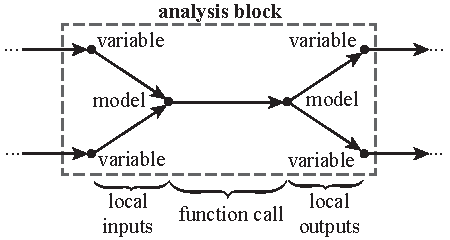
\includegraphics[width=4in]{images/analysis_block}
	\end{center}
	\vspace{-10pt}
\caption{Example analysis block. The each node type and edge type is labeled in italics and annotated parenthetically.}
\label{f:analysis block}
\end{figure}
%`Connection' edges connect the local outputs from one analysis block to input nodes.

\section{Graph--based Representation of the Fundamental Problem Formulation}
Next we provide the meaningful graphs that can be created from the suggested syntax. The first graph is the \emph{maximal connectivity graph} which represents the full potential of all the analysis codes being considered, i.e. each analysis code is represented by an analysis block, and each potential connections between variables is represented by a free edge. The second graph that may be represented is \emph{fundamental problem formulation graph}, which is the graph with the fewest number of edges and nodes needed to provide a valid problem formulation, as disscussed subsequently. Finally, a \emph{solution problem formulation} may be represented by including additional edges and node times to represent the optimization architecture, though this is beyond the scope of this paper. 

The relationship between these three graphs is depicted in Figs.~\ref{f:tree} and \ref{f:hourglass}. The tree diagram demonstrates the fact that it is generally possible to obtain multiple FPFs from a single maximal connectivity graph. This  may correspond to different down--selections of analysis codes, different connections between them, or both. Then, for each FPF, different SPFs may be obtained by implementing different optimization architectures. The hourglass shape indicates that the FPF graph is the smallest graph that may represent a specific problem formulation. The FPF is obtained from the MCG by removing nodes and edges, and the SPF is obtained from the FPF by adding nodes and edges.
\begin{figure}[htb!]
	\centering
	\subfigure[number of possible graphs]{
	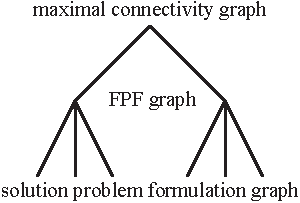
\includegraphics[width=2.0in]{images/tree}
	\label{f:tree}
	}
	\subfigure[graph size]{
	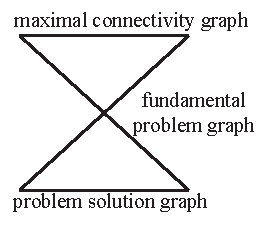
\includegraphics[width=2.0in]{images/hourglass}
	\label{f:hourglass}
	}
\caption{The relationship between the MCG, FPF, and SPF.}
\end{figure}

In this section we introduce the remaining necessary notion and give graph--theory based definitions of the MCG and FPF, and then process to demonstrate how the FPF is obtained from the MCG.

\subsection{Additional Notation}
For node $v \in V$ the edges directed out are given by $E(v)$ and the edges directed into $v$ are given by $E^{-1}(v)$; $E(E(v))$ is denoted as $E^2(v)$, and likewise for additional levels. 
The \emph{indegree} of a node is the number of edges directed in and is denoted as $\txt{deg}^-(v)$, and the \emph{outdegree} is the number of edges directed out and it is denoted as $\txt{deg}^+(v)$.
We also define the \emph{upper indegree limit} 
\begin{equation}
\txt{deg}_u^-(v):V \to \mathbb{N}
\end{equation} 
and the \emph{lower indegree limit}
\begin{equation}
\txt{deg}_l^-(v):V \to \mathbb{N}.
\end{equation}
These user-specified limits set the number of edges that may be directed into a node for a problem formulation to be valid. For example, a variable node $v$ will have $\txt{deg}_u^-(v) = \txt{deg}_l^-(v) = 1$, unless it is a multi--fidelity variable, in which case the user may specify some upper limit higher than one.

To keep track of which nodes and edges are which type, let $T_\txt{node}$ and $T_\txt{edge}$ be sets containing the possible node types and edge types, respectively, and then define mappings $t_\txt{node}:V \to T_\txt{node}$ and $t_\txt{edge}:E \to T_\txt{edge}$ to assign a type to each node and edge.
Then, for example, for a variable node $v$ we have $t_\txt{node}(v) = \txt{`variable'}$.


 % A \emph{path} is a nonempty graph $P = (V,E)$ with $V = \{x_0,x_1,\ldots,x_k\}$ and $E = \{x_0x_1,x_1x_2,\ldots,x_{k-1}x_k\}$, where $x_i$ are all distinct. A graph $G$ is \emph{connected} if any two of its vertices are linked by a path in $G$. A \emph{tree} is a connected and acyclic graph.
%%% this needs to be changed to fit the definition using a directed graph


\subsection{Maximal Connectivity Graph}
To construct the maximal connectivity graph, we assume that a set of codes, global inputs, and objectives and constraints (collectively called global outputs). The codes are represented by analysis blocks $A_i=(V_{A_i},E_{A_i}), \ i=1,\ldots,m$, the global inputs are represented a set of variable nodes $I$, and the global outputs are represented by a set of variable nodes $O$. We assume that $O$, $I$, and $A_i$ are given, and that any potential connection between variables is given in the form of the free edges in the set $C_M$. 
Then we may construct the maximal connectivity graph $M=(V_M,E_M)$ as
\begin{IEEEeqnarray*}{rCl}
V_M & = & I \cup O \cup \left( \bigcup_{i = 1}^m V_{A_i} \right), \\
E_M & = & C_M \cup \left( \bigcup_{i=1}^m E_{A_i} \right),
\end{IEEEeqnarray*}
The MCG $M$ is uniquely determined by the given set of analysis blocks, the required outputs, and the given global inputs. In the cases where the set of global inputs $I$ is not known a priori, the process of obtaining the FPF will reveal the required inputs, as discussed subsequently.

\subsection{Fundamental Problem Formulation Graph}
We now define the fundamental problem formulation graph, $F=(V_F,E_F)$, as a directed graph meeting the following conditions
\begin{enumerate}
\item[(1)] $\displaystyle{V_F = I_F \cup O \cup \left( \bigcup_{i \in \mathcal A} V_{A_i} \right),\ I_F \subset I}$
\item[(2)] $\displaystyle{E_F = C_F \cup \left( \bigcup_{i \in \mathcal A} E_{A_i} \right)}$
\item[(3)] $\displaystyle{\forall v \in V_F \txt{ with } t_\txt{node}(v) = \txt{`variable,'}\quad \txt{deg}_l^-(v) < \txt{deg}^-(v) \leq \txt{deg}_u^-(v)}$
\end{enumerate}
The set $\mathcal A$ is an index set containing the indices of the analysis blocks in $F$; for the case where all of the analysis blocks are used, we would have $\mathcal A = \{1,2,\ldots,m\}$. The first requirement for $F$ is that $V_F$ be composed of all of the global outputs (the required objectives and constraints), the nodes from each analysis block in $F$, and any global input nodes that are needed, $I_F$. The second requirement suggests that the edges in $F$ comprise the edges for each analysis block and the edges between them, the global inputs, and the global outputs. The final requirement is specific to the number of edges directed into a variable. If there are no edges directed inward, the node is called a \emph{hole}, and if more connections are directed in than are allowed, the node is called a \emph{collision}; a hole is allowed if $\txt{deg}_l^-(v)=0$. The final requirement is therefore a requirement on $C_F$.

\subsection{Obtaining the Fundamental Problem Formulation Graph}
In general, there may be multiple different graphs that satisfy the FPF conditions, though there may be none at all. Here, we describe a process for obtaining an FPF by starting with the MCG and disconnecting free edges until the FPF conditions are met. Then the problem is reduced to deciding which free edges to remove.

%Then, mathematically, the FPF starts with $\mathcal A_1 = \{1,\ldots,m\}$, $I_{F,1} = I$, and $C_{F,1} = C_M$.
Then, mathematically, the FPF starts with $C_{F,0} = C_M$.
First address the nodes where $\txt{deg}^-(v) < \txt{deg}_l^-(v)$ then the ones where $\txt{deg}^-(v) > \txt{deg}_u^-(v)$

\begin{enumerate}
\item The first step is to detect holes and disconnect the free edges following them. These free edges are removed because they represent variables which cannot be determined because the analysis function does not have adequate inputs. The set of variable nodes which are holes is created as
\begin{equation}
H = \{v \in V | \txt{deg}^-(v) < \txt{deg}_l^-(v) \}
\end{equation}
Then the updated set of edges is
\begin{equation}
C_{F,1} = C_{F,0} \setminus \{\ e \in E, \ e=xy | x=E^3(v) \txt{ for } v \in H\}
\end{equation}
%deg-v is now recaculated for the new C. 
This step is demonstrated by Fig.~\ref{f:holes}.
\item (())
\end{enumerate}
\begin{figure}[htb!]
	\begin{center}
	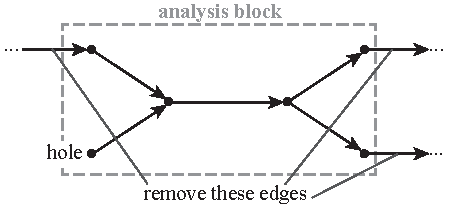
\includegraphics[width=3in]{images/analysis_block_hole}
	\end{center}
	\vspace{-20pt}
\caption{Example variable node indicating a hole.}
\label{f:holes}
\end{figure}


%\begin{enumerate}
%\item The first step is to detect holes and remove the corresponding analysis blocks, which could not be used because the required inputs are not supplied. Any analysis blocks with holes may be stored in an index set $\mathcal H$ as
%\begin{equation}
%\forall i \in \mathcal A_1,\txt{ and }\forall v \in V_{A_i},\txt{ if deg}^-(v)=0 \txt{ then } i \in \mathcal H.
%\end{equation}
%Then an updated index set $\mathcal A_2$ is created using set difference notation as
%\begin{equation}
%\mathcal A_2 = \mathcal A_1 \setminus \mathcal H
%\end{equation}The connection edges directed from the removed analysis blocks are removed as
%\begin{equation}
%H = \{c \in C_{F,1} |c = (e^{-1}(v),v), \txt{ where } v \in V_{A_i} \txt{ for some } i \in \mathcal H\},
%\end{equation}
%\begin{equation}
%C_{F,2} = C_{F,1} \setminus H
%\end{equation}
%Finally, the FPF is updated as
%\begin{equation}
%V_{F,2} = I_{F,2} \cup O \cup \left( \bigcup_{i \in \mathcal A_2} V_{A_i} \right),
%\end{equation}
%\begin{equation}
%E_{F,2} = C_{F,2} \cup \left( \bigcup_{i \in \mathcal A_2} E_{A_i} \right)
%\end{equation}
%This process may require multiple iterations because removing an analysis block may create holes upstream. It is assumed that the process as been repeated sufficiently such that $\mathcal A_2$ does not have any holes.
%
%\item The next step is to resolve conflicts. The set $C$ of input nodes containing conflicts is
%\begin{equation}
%C = \{v \in V_{F,2} | t_\txt{node}(v) = \txt{`input'} \txt{ and } \txt{deg}^-(v) > d(v)\}
%\end{equation}
%%\begin{equation}
%%for v \in c let 
%%\end{equation}
%\end{enumerate}

%\subsection{Classification of the FPF}

%A collision represents a choice.
%Delete edges and analysis blocks so that there are no nodes or collisions.





% \begin{figure}[htb!]
	% \begin{center}
	% 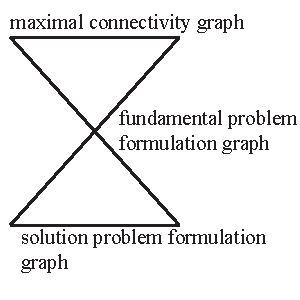
\includegraphics[width=2in]{images/hour_glass}
	% \end{center}
	% \vspace{-20pt}
% \caption{(()).}
% \label{f:our glass}
% \end{figure}
% \subsection{old}
	% For a large scale problem with many analyses, obtaining the FPF is likely to be a challenge. In general, a set of analysis codes will be given and the desired outputs will be specified as
	    % \begin{align}
            % given & \ \ A: \lbrace x_i \lvert i \in A_\textrm{input} \rbrace \rightarrow \lbrace x_i \lvert i \in A_\textrm{output} \rbrace \notag
            % \\    & \ \ B: \lbrace x_i \lvert i \in B_\textrm{input} \rbrace \rightarrow \lbrace x_i \lvert i \in B_\textrm{output} \rbrace \notag
			% \\    & \ \ \quad \quad \quad \quad \quad \quad  \quad \quad \vdots
            % \\min. &\ \ f(x_i), i \in \mathcal{O} \notag
            % \\w.r.t. & \ \ x_i, i \in \mathcal{I}, \notag
            % \label{eqn:preFPF}
        % \end{align}
	% where $\mathcal{O}$ is the index set of the global outputs and $\mathcal{I}$ is the index set of the global inputs. For this to be an FPF, there must be no \emph{conflicts} or \emph{holes}. A conflict arises when different analyses produce the same output; two analysis codes $A$ and $B$ are in conflict if
		% \begin{equation}
			% A_\textrm{output} \cap B_\textrm{output} \neq \emptyset.
		% \end{equation}
	% A hole arises when a local input to an analysis block is neither a global input nor a local output of any analysis block. If we let $\mathcal{H}$ denote the index set of local inputs which are holes
		% \begin{equation}
			% i \in \bigcup \{A_\textrm{input},B_\textrm{input},\ldots\} \textrm{ and } i \notin \bigcup \{\mathcal{I},A_\textrm{output},B_\textrm{output},\ldots\}  \implies  i \in \mathcal{H}.
		% \end{equation}
	% If the given set of analyses contains any holes, an FPF cannot be obtained. On the contrary, if there are conflicts multiple FPFs may be obtained. This is because every conflict represents a choice of which analysis to use and each choice could (potentially) yeild a different but valid FPF. The following section develops an application of graphy theory to obtain multiple FPFs from a set of analyses and desired outputs.
		
    % \subsection{Formulation Graph Syntax}
    % Rather than start with an adjacency, we chose to work directly with a directed cyclic graph to develop a syntax for the FPF. 
    % The following information must be provided to start:
    % \begin{itemize}
        % \item Analysis blocks: an analysis block represents any calculation, and each comes with
            % \begin{itemize}
                % \item local inputs
                % \item local outputs 
                % \item execution properties: these are the properties associated with running the code, such as run time
            % \end{itemize}
        % \item Global parameters: these may serve as fixed inputs to the local inputs of analysis blocks
        % \item Global outputs: these may represent
            % \begin{itemize}
                % \item objectives
                % \item constraints
                % \item residuals: (not sure)
            % \end{itemize}
    % \end{itemize}

    % The graph representation of a data flow is cast to utilize the extensive library of algorithms in graph theory to analyze a directed weighted graph. 
    % Edge weights are used to represent the metrics associated with a data flow:
    % \begin{itemize}
        % \item Run time: this metric is a property of an analysis block
        % \item Fidelity: this metric is a property of an individual local output
        % \item Expected Convergence
    % \end{itemize}

    % The key assumption is that identical variables are recognized as such. This serves as the basis for creating a data flow by connecting compatible input and output nodes with a directed edge. 
    % To represent the fact that execution of an analysis code does not depend on the number of outputs being used, we have created the following figure (not made yet).
    
    % This information immediately leads to the maximal connectivity graph, which is formed by placing a directed edge from each local output or global parameter to each matching local input or global output. 
    % Whenever multiple edges are connected to a single input, a conflict occurs because only one may be used. Resolving these conflicts is one key challenge in creating a data flow.
%    \begin{itemize}
%        \item Specify analyses
%        \item Connections between analyses 
%            \begin{itemize}
%                \item local variables
%                \item global variables? Use "fake" node that broadcasts out to the rest of the graph? 
%            \end{itemize}
%        \item Cycles indicate coupling
%        \item Cycles for design variables->objectives/constraints
%        \item Objectives/constraints are just outputs? Special nodes? 
%        \item Residuals are just outputs? Special nodes? 
%        \item Parameters are just input nodes that are not design variables (use identifies these)
%        \item FPF no solvers/optimizers anywhere in it
%    \end{itemize}

    \subsection{Solution Graph Syntax}
    What is the difference between a problem formulation and a problem solution method? Convert from a cyclic graph, to an acyclic graph
    \begin{itemize}
        \item Cycles indicate convergence loops or design variable loops
        \item Problem can't be solved until all loops are *removed* by adding solvers/optimizers
        \item *Special* nodes for solvers and optimizers that *break* loops (from an algorithmic point of view)
        \item FPF represents the minimal amount of information necessary to define a problem
        \item Any solution path grows the graph complexity by adding edges and nodes (or possibly have an empty solution graph, which you build up
        as you remove edges from problem formulation graph?)
    \end{itemize}


    
\section{Example Problem}

\section{Applications}

\section{Conclusions}

\bibliography{library}
\end{document}